\section{Monitor \& Controlling Process Group}
Ora dobbiamo controllare che il piano finora sviluppato venga rispettato. Monitoraggio e controllo non sono sinonimi.
\begin{itemize}
	\item \textbf{Monitoraggio} significa raccogliere dati, i quali vengono utilizzati per verificare se il progetto sta venendo svolto nel modo corretto. Il piano, anche denominato "baseline" ci fornisce indicazioni su cosa significhi "modo corretto".
	\begin{info}
		Essere in baseline significa "star rispettando il piano" o "essere al passo col piano". Se un'attività per esempio sta venendo svolta in ritardo rispetto ad una tabella di marcia allora non siamo in baseline e bisogna cercare di recuperare.
	\end{info}
	\item Controllo significa fare qualcosa, ovvero portare una situazione in una fase accettabile secondo il piano. Non serve intervenire non appena si verifica un lieve ritardo. Esistono dei valori soglia che ci indicano quando conviene intervenire. In alcuni casi il motivo dei ritardi è chiaro, in altri serve capire le cause per poter trovare le contromisure. Anche "non fare niente" è un'opzione accettabile a volte.
\end{itemize}

\subsection{Tools, templates e processi per monitorare e controllare il progetto}
La maggior parte dei tool nella fase di monitoraggio consiste in report.
\begin{itemize}
	\item \textbf{Current period reports}: focalizzati sul lavoro di un certo periodo di tempo corrente. Coprono solo i periodi più recenti del progetto. Evidenziano le attività completate più rilevanti e le eventuali variazioni rispetto a quanto pianificato. Possono anche includere un’analisi delle ragioni che hanno causato le eventuali variazioni e sulle corrispondenti misure correttive. In Scrum il periodo potrebbe essere anche il tempo di uno sprint. Sconsigliato un periodo troppo breve come "un giorno" perché l'overhead aumenta. Una base settimanale può essere un buon periodo;
	\item \textbf{Cumulative reports}: focalizzati sull'andamento del progetto (dall'inizio). Coprono l’intera storia del progetto e sono molto efficaci nel mostrare i trend nell’avanzamento del progetto. Per esempio, possono essere tracciati tutti gli scostamenti rispetto al pianificato e rilevare se la “situazione” sta migliorando o peggiorando;
	\item \textbf{Exception reports}: focalizzati principalmente su problemi o su attività problematiche. Sono rivolti al senior management e si concentrano sulla descrizione degli scostamenti rispetto al pianificato, delle cause e delle misure correttive da intraprendere. Sono molto sintetici e tuttalpiù prevedono degli allegati con maggiori dettagli;
	\item \textbf{Stoplight reports}: focalizzati per esempio sui colori, offrono un approccio visuale molto comodo per capire se si è in tempo con determinate attività oppure no. Possono essere visti come una variante applicata ai report di tipo current period, cumulative ed exception. Puntano a segnalare al senior management in modo estremamente sintetico lo stato di avanzamento del progetto. Per esempio, si può pensare di aggiungere agli altri tipi di report delle note con supporti visuali (e.g., post-it) per identificare rapidamente delle situazioni.
	\begin{info}[Esempio dell'utilizzo dei colori in stoplight]
		\item \textit{Verde}: “tutto procede come pianificato”;
		\item \textit{Giallo}: “vi sono stati scostamenti ma è tutto sotto controllo”;
		\item \textit{Rosso}: “situazione fuori controllo”. Una riunione in questo caso è quasi sempre necessaria.
	\end{info}
	Utilizzare pochi colori rende semplice capire le situazioni, aggiungerne rende più specifiche le situazioni ma rende più difficile l'identificazione rapida del problema;
	\item \textbf{Variance reports}: focalizzati sulle variazioni, sulle differenze. Concentrano la loro attenzione sugli scostamenti rispetto al pianificato. Per ogni attività e periodo riportano il confronto tra quanto pianificato e lo stato di avanzamento effettivo. Per riportare le informazioni possono essere utilizzate sia delle tabelle che dei grafici;
	\item \textbf{Gantt charts}: durante questa fase diventa strumento di monitoraggio perché grazie a questo è possibile capire la situazione delle attività attuali rispetto a quella prevista;
	\item \textbf{Burn charts}: focalizzato su quanto lavoro manca. Si misura il lavoro come un "qualcosa che va bruciato" e si finisce quando tutto è stato bruciato;
	\item \textbf{Milestone trend charts}: focalizzato sull'andamento delle milestone;
	\item \textbf{Earned value analysis}: lo strumento sulla carta più quantitativo. C'è l'idea di cercare di capire quale valore stiamo recuperando. Verrà approfondito in seguito;
	\item \textbf{Integrated milestone trend charts and earned value analysis}: mix delle due precedenti soluzioni;
	\item \textbf{Project status meetings}: qualsiasi tipo di meeting è anche monitoraggio, dallo stand-up meeting al meeting di fine di uno sprint in scrum;
	\item \textbf{Problem escalation strategies}: un metodo di controllo in cui si chiede aiuto in "ordine gerarchico" fino a quando il problema non viene risolto. Per esempio il team prova a risolvere il problema prima di chiedere aiuto ad un livello più alto.
\end{itemize}
\subsubsection{Rispettare la Schedula di progetto}
Per mantenere il progetto entro i binari stabiliti in fase di pianificazione, secondo le buone pratiche è necessario:
\begin{itemize}
	\item \textbf{Tenere dei daily team meetings}: per riuscire a risolvere problemi prima che diventino troppo grandi per poter essere risolti efficacemente;
	\item \textbf{Completare i tasks il prima possibile};
	\item \textbf{Riportare eventuali problemi il prima possibile};
	\item \textbf{Non essere vittima delle “creeps”}: Ricordiamo che le creeps sono quei cambiamenti lievi ed impercettibili ed insidiosi, ma quando i loro effetti si accumulano possono diventare problemi importanti;
	\item \textbf{Non provare a indovinare: nel dubbio bisogna fare domande};
	\item \textbf{“Good enough is good enough”}: se non lavoriamo per avere eccellenza ma lavoriamo che fare in modo che tutto funzioni e basta il risultato finale sarà medio. Mantenere un passo costante e cercare di minimizzare il debito tecnico devono sempre essere questioni centrali;
	\item \textbf{Rispettare i requisiti, ma non andare oltre i requisiti (rischio di overdesign)}: overdesign significa aggiungere qualcosa di non richiesto o non gradito;
	\item \textbf{Bisogna essere aperti e onesti con i propri colleghi del team}: mentire significa sabotare il sistema di monitoraggio. Spesso si pensa che tenere nascosto qualcosa nella speranza che si risolva il prima possibile sia meglio che ammettere di essere in ritardo.
\end{itemize}

\subsection{Sistema di reporting}
\subsubsection{Effective Progress Reporting}
Per effettuare in modo efficiente il reporting sullo stato di avanzamento del progetto è consigliabile dotarsi di un sistema di supporto (Progress Reporting System), che dovrebbe avere le seguenti caratteristiche:
\begin{itemize}
	\item \textbf{Fornire informazioni sullo stato di avanzamento tempestive, complete e accurate}: uno dei problemi dei sistemi di rendicontazioni è che inserire a fine orario di lavoro le entry su cosa è stato fatto durante la giornata non è divertente e spesso viene posticipato, causando problemi come la perdita di informazioni se non la completa assenza. Inoltre non avere inserimenti costanti non permette di fare monitoraggio costante, causando ritardi in processi di controllo;
	\item \textbf{Non deve richiedere un “overhead” eccessivo per il suo utilizzo (in termini di effort), tanto da essere controproducente}: sarebbe ideale avere un sistema di rendicontazione automatico ma è praticamente impossibile. Possibile invece è avere a disposizione un sistema reattivo e rapido da usare, anche perché utilizzare troppo tempo per la rendicontazione ne toglie al lavoro effettivo;
	\item \textbf{Il reporting deve essere intuitivo e facilmente accettabile da parte del team di progetto e del senior management}: la curva di apprendimento deve essere molto bassa, serve il clima aziendale adatto per capire che il tool viene utilizzato per aiutare e non per giudicare. Prima si trova il problema e prima si recupera;
	\item \textbf{Il sistema deve essere un efficace strumento per poter avere un allarme tempestivo (early warning) se ci fossero dei problemi a rispettare quanto pianificato}.
\end{itemize}
\subsubsection{Come e quali informazioni aggiornare}
\begin{enumerate}
	\item Prima di tutto bisogna determinare i periodi da monitorare (e.g., settimana) e per ognuno di questi bisogna definire in quale giorno e ora aggiornare le informazioni (e.g., un particolare giorno della settimana e un orario ben preciso). Parola chiave di questo processo è consistenza;
	\item Riportare il lavoro effettivamente svolto durante il periodo in esame in modo fedele;
	\item Registrare tutti i dati storici sull’eseguito nei periodi precedenti e aggiornare le stime sulle attività rimanenti. Utile per mantenere visione su cosa è stato fatto e cosa rimane da fare;
	\item Riportare le date di inizio e fine di ciascuna attività iniziata o terminata nel periodo in esame;
	\item Registrare i giorni già impegnati su ciascuna attività e quelli previsti per il completamento;
	\item Riportare le risorse consumate e quelle rimanenti;
	\item Riportare la percentuale di completamento. Problematico perché la "definizione di DONE" permette di capire bene quando un'attività è stata completata al 100\%, ma difficile fornire valori intermedi. Una possibilità è fornire un peso ad ogni test.
\end{enumerate}

\subsection{Strumenti di reporting visuale}

\subsubsection{Gantt Chart Project Status Report}
Ogni riga nel Gantt è un'attività. Ogni barra ci dice quando l'attività dovrebbe iniziare e quando dovrebbe finire. Nell'immagine che segue la linea tratteggiata indica il giorno corrente. Attraverso il sistema di rendicontazione è anche possibile avere un'indicazione proprio sul Gantt per capire come stanno andando le attività.
\centeredImage{document/img/ganttchart.png}{Gantt Chart Project Status Report}{0.6}

\subsubsection{Cumulative Reports - Milestone Trend Charts}
I Cumulative Report che seguono sono stati organizzati mettendo sulle ascisse i mesi di progetto. Se il puntino di ogni mese rimane su un valore di \textit{y} uguale a 0 allora siamo in schedula. Se il valore di \textit{y} è maggiore di 0, per esempio è 1, allora siamo in anticipo di un mese rispetto ai tempi. Se il valore di \textit{y} è sotto lo 0, ad esempio è -2, siamo in ritardo di due mesi. In questi cumulative report mancano informazioni sulle ragioni di anticipi e ritardi. Il Cumulative Report ci fornisce indicazioni su come sta andando il progetto rispetto al passato.\newline

\noindent Prendiamo in considerazione l'immagine \ref{cumreport1}. Capiamo facilmente che il progetto di questo cumulative report sta andando male e i ritardi continuano ad aggiungersi. In questi casi bisogna assolutamente capire cosa non sta funzionando e perché. Un buon Project Manager avrebbe dovuto agire intorno al terzo o quarto mese. In alcuni casi questa situazione può anche essere tollerabile, ma devono esserci motivazioni valide.
\begin{figure}[H]
	\centering
	\begin{subfigure}[b]{0.45\textwidth}
		\centering
		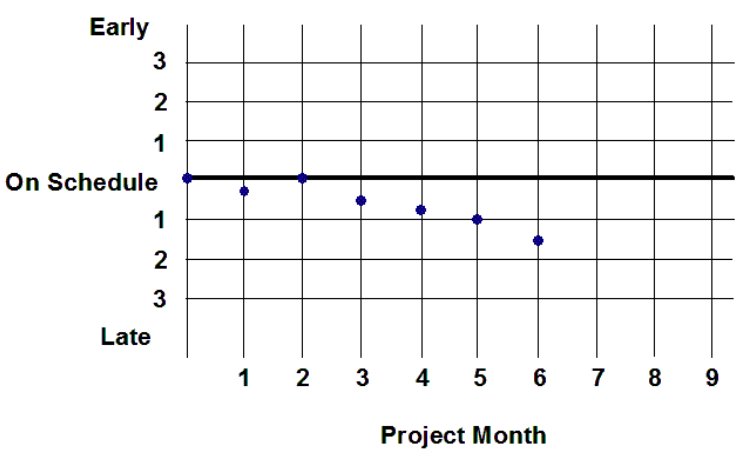
\includegraphics[width=\textwidth]{document/img/cumreport1.png}
		\caption{Cumulative Report \#1}
		\label{cumreport1}
	\end{subfigure}
	\hfill
	\begin{subfigure}[b]{0.45\textwidth}
		\centering
		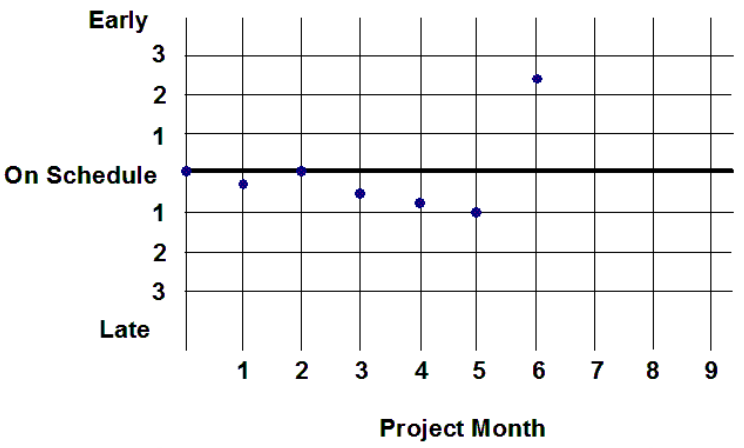
\includegraphics[width=\textwidth]{document/img/cumreport2.png}
		\caption{Cumulative Report \#2}
		\label{cumreport2}
	\end{subfigure}
	\caption{Esempi di Cumulative Reports}
\end{figure}

\noindent Nell'immagine \ref{cumreport2} invece nel giro di un mese la situazione è migliorata moltissimo. Questo può essere dovuto ad una contromisura come l'aggiunta di molto personale o la rimozione di molti requisiti. Una volta apportate le contromisure è stato rivalutato il piano. Secondo i nuovi parametri quindi lo stato di avanzamento del progetto è molto in anticipo. Guardando solo questo grafico la situazione dei ritardi sembra migliorata notevolmente, ma non sappiamo cosa è peggiorato per portarci a questa situazione. È sempre una questione di compromessi.\newline

\noindent Nell'immagine \ref{cumreport3} il progetto parte subito in anticipo dai primi mesi. In questo caso SOLO le attività del primo mese sono state valutate in modo pessimistico, infatti una volta portate a termine la situazione rimane abbastanza costante. Probabilmente si è preferito stare larghi, ad esempio a causa di fattori di rischio (come una nuova tecnologia). Per il resto tutto sta procedendo come pianificato. Il mese guadagnato finisce nella scope bank.\newline

\noindent Nell'immagine \ref{cumreport4} c'è stato un rework generale tra il mese 3 e il mese 4 che ha portato una situazione tutto sommato buona ad una ancora migliore grazie a dei miglioramenti improvvisi.

\begin{figure}[H]
	\centering
	\begin{subfigure}[b]{0.45\textwidth}
		\centering
		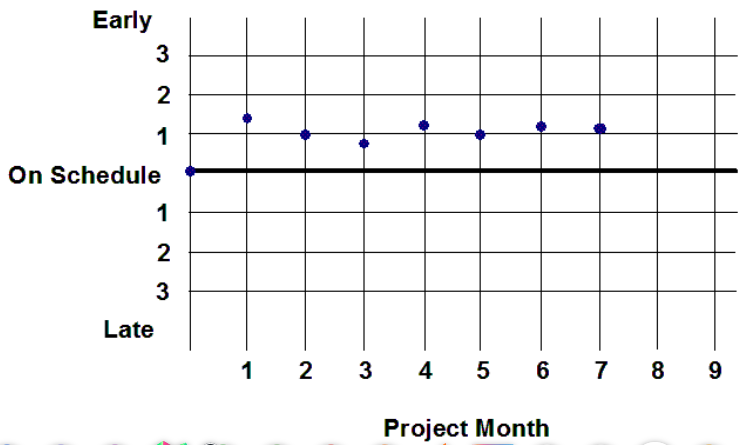
\includegraphics[width=\textwidth]{document/img/cumreport3.png}
		\caption{Cumulative Report \#3}
		\label{cumreport3}
	\end{subfigure}
	\hfill
	\begin{subfigure}[b]{0.45\textwidth}
		\centering
		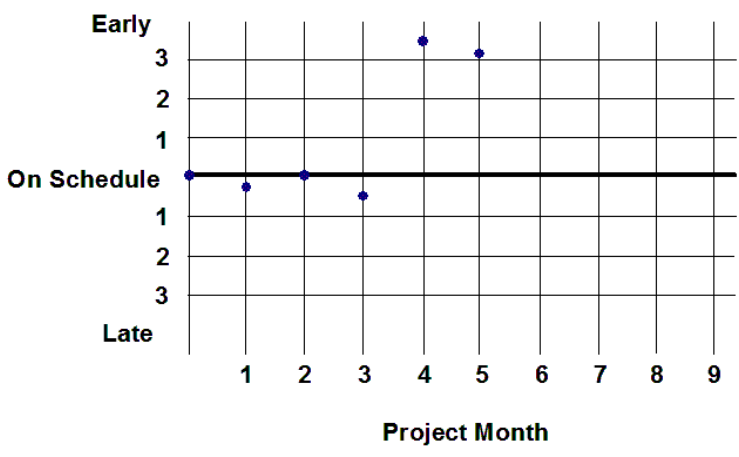
\includegraphics[width=\textwidth]{document/img/cumreport4.png}
		\caption{Cumulative Report \#4}
		\label{cumreport4}
	\end{subfigure}
	\caption{Altri esempi di Cumulative Reports}
\end{figure}

\subsubsection{Earned value}
Il problema dei cumulative report è che ci si concentra principalmente sul tempo, quando in realtà esistono due grandezze principali che sono legate tra loro: tempo e costi. Sarebbe utile avere degli indici che le riguardano, piazzando nelle \textit{x} il tempo e nelle \textit{y} i progressi.

\noindent La situazione classica è quella di una funzione logistica in cui si parte in modo abbastanza tranquillo, per poi arrivare in produzione, ovvero il punto in cui il valore aumenta sempre di più, fino ad arrivare alla fine in cui ci sono le piccole cose da fare e quindi il valore diminuisce fino a stabilizzarsi. Questo significa che il completamento del progetto è vicino. È abbastanza usuale che la parte più produttiva sia quella centrale.

\centeredImage{document/img/s-curve.png}{Classica S-curve}{0.4}

\noindent Potremmo anche avere un progetto che parte subito, in cui la situazione è ottimale e produciamo subito valore, magari perché abbiamo dimestichezza con il dominio o le tecnologie.

\centeredImage{document/img/aggressive-curve.png}{Aggressive Curve}{0.4}

\noindent La situazione potrebbe anche essere più complessa ovviamente. In questo caso il momento in cui si impiega a raggiungere la produzione è più lungo. Classico il caso in cui è necessario lavorare sull'infrastruttura che fa da bottleneck e impedisce all'utente di capire quanto valore si può allocare nel progetto. Anche in questo caso però non bisognerebbe fare l'errore di attribuire troppo peso al valore, perché potrebbe risultare in problemi all'infrastruttura che magari proprio per sua natura richiede tanto tempo per essere creata.

\centeredImage{document/img/curve-to-avoid.png}{Curve to Avoid}{0.4}

\noindent Il lavoro effettivamente svolto è confrontato con il lavoro previsto dal piano, per determinare gli scostamenti rispetto alla schedula e ai costi previsti.\newline
L’impiego del valore economico o del tempo/uomo non sono ideali. I teorici suggeriscono infatti di non usare tempo e denaro come assi nei grafici appena illustrati. Tuttavia nessuno è ancora riuscito a trovare un'alternativa valida.\newline
Il limite è che questi strumenti non danno indicazioni sulle motivazioni e pertanto non sono sufficienti per formulare delle valide previsioni per il futuro.

\noindent Il valore infatti può anche essere un incremento del livello di servizio per l'azienda, che avrà ripercussioni future. In alcune situazioni, come i progetti sostenibili il valore viene spesso restituito alla comunità piuttosto che ottenuto.

\begin{info}[Come misurare l'earned value:]
	Esiste il solito problema in cui bisogna portare a termine un certo numero di attività. In questo esempio ci sono 14 attività. Come possiamo determinare la percentuale di completamento di quella feature?\newline
	Se la feature richiede 14 attività e ne abbiamo completate 10 potremmo pensare di rapportare i due valori, ma questo è possibile solo se le attività hanno tutte lo stesso peso. Un calcolo pesato potrebbe essere una soluzione migliore, ma non sempre è una buona idea. Spesso nella realtà non si ragiona in scala di grigi ma in bianco e nero. Si attribuisce il 100\% solo quando un'attività rispetta la definizione del "DONE" e 0\% altrimenti. A volte anche il 50\% viene aggiunto per avere un livello di dettaglio in più.
	\centeredImage{document/img/earned-perc.png}{Misurare l'earned Value percentuale}{0.3}
\end{info}

\subsubsection{Cost e Schedule Variance}
Nell'immagine che segue, la linea verde denotata con "Baseline" rappresenta il piano. Si tratta dell'indicazione che dovrebbe essere seguita, sostanzialmente si tratta di un punto di riferimento.
La curva rossa denotata con "Actual" rappresenta ciò che è realmente successo.

\paragraph{Cost Variance}
In questo caso il valore assunto dalla \textit{y} nell'istante temporale attuale è differente rispetto a quello della baseline. La differenza tra i due prende il nome di Cost Variance. Il nome è dovuto dal fatto che questa indicazione potrebbe essere vista come una differenza tra quello che siamo riusciti a generare come valore e quello che il piano ci diceva di generare. Il fatto che ci sia differenza non ha necessariamente un impatto sui costi.
\centeredImage{document/img/cost-variance.png}{Cost Variance}{0.45}

\paragraph{Schedule Variance}
Se valutiamo la situazione  prendendo in considerazione lo stesso livello di progresso possiamo valutare la differenza temporale tra la baseline e la situazione attuale. Questo valore prende il nome di Schedule Variance.
\centeredImage{document/img/schedule-variance.png}{Schedule Variance}{0.5}

\subsubsection{Come misurare l'earned value}
Il \textit{planned value (PV)} è il valore contenuto nel piano. Ad esempio si è stimato che completare un attività di 5 giorni costa 500 dollari.\newline
L'\textit{earned value (EV)} è il vero valore effettivamente guadagnato. Avendo iniziato a lavorare tardi abbiamo ottenuto nell'arco di 5 giorni solo 300 dollari e non 500 perché non ne abbiamo usati 2.\newline
L'\textit{actual value (AC)} è invece ciò che è davvero successo. Anche se partiti in ritardo sono già stati spesi 100 dollari in più rispetto ai piani. Questa è proprio la cost variance, ovvero la differenza di costi rispetto alla baseline. Per ottenere lo stesso valore sto quindi spendendo di più.
\centeredImage{document/img/measure-earned-value.png}{Misurare l'earned value}{0.5}

\noindent A questo punto abbiamo le informazioni che ci permettono di predire cosa accadrà. In caso di ritardi avremo uno slittamento in lunghezza. Si verifica anche uno slittamento in altezza perché si ha un generale incremento nei costi.
\centeredImage{document/img/the-full-story.png}{The full Story - Curve}{0.5}

\noindent Attraverso queste misure è possibile calcolare dei nuovi indici:
\begin{itemize}
	\item \textbf{Schedule Performance Index (SPI)}: Fornisce una misura di come il progetto sta performando rispetto a quanto pianificato. Si calcola nel seguente modo: $SPI = \frac{EV}{PV}$;
	\item \textbf{Cost Performance Index (CPI)}: Fornisce una misura di come i costi del lavoro svolto evolvono rispetto ai costi di progetto stimati in fase di pianificazione. Si calcola nel seguente modo: $CPI = \frac{EV}{AC}$.
\end{itemize}
I valori che possono assumere gli indici sono:
\begin{itemize}
	\item \textbf{< 1}: oltre il budget o in ritardo rispetto alla schedula prevista;
	\item \textbf{> 1}: sotto il budget o in anticipo rispetto alla schedula prevista.
\end{itemize}
\centeredImage{document/img/pv-ev-ac.png}{PV EV e AC curves}{0.45}

\noindent Questi indici possono essere inseriti in dei report grafici. L'asse delle \textit{x} ancora una volta rappresenta il tempo mentre quello delle \textit{y} il valore assunto dagli indici. Se il valore resta sempre intorno all'1 significa che si sta rispettando perfettamente il piano. Nell'immagine \ref{perfind1} va tutto secondo i piani fino ad un certo punto, finché drammaticamente peggiora la situazione e si aggiunge del ritardo (S), ma possiamo notare che stiamo comunque spendendo poco rispetto al pianificato (C). In questo caso forse non è stato attribuito "tempo pieno" al progetto, magari perché nel frattempo ne sono subentrati altri. In ogni caso per approfondire le cause del problema sarebbe opportuno fare una riunione coi responsabili delle attività in ritardo (li possiamo trovare nel GANTT ad esempio).

\noindent Nell'immagine \ref{perfind2} si parte in modo abbastanza costante, ma ad un certo punto si cominciano a guadagnare tempo e costi in modo abbastanza costante. In questo caso la causa potrebbe essere dovuta al pessimismo nelle stime, ma potrebbe anche essere a causa del team che migliora.

\begin{figure}[H]
	\centering
	\begin{subfigure}[b]{0.45\textwidth}
		\centering
		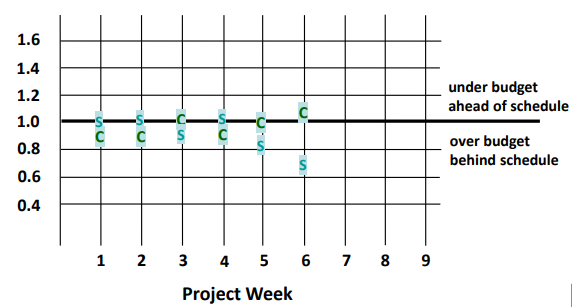
\includegraphics[width=\textwidth]{document/img/performance-indices-1.png}
		\caption{Indici di performance \#1}
		\label{perfind1}
	\end{subfigure}
	\hfill
	\begin{subfigure}[b]{0.45\textwidth}
		\centering
		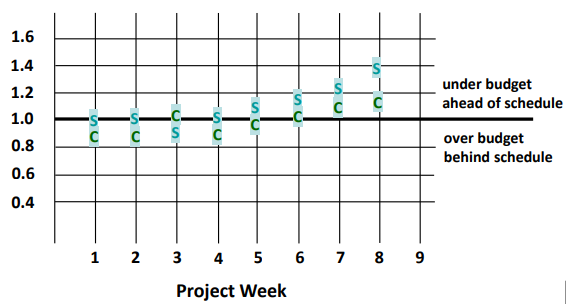
\includegraphics[width=\textwidth]{document/img/performance-indices-2.png}
		\caption{Indici di performance \#2}
		\label{perfind2}
	\end{subfigure}
\end{figure}

\noindent Nell'immagine \ref{perfind3} abbiamo la situazione opposta. Anche in questo caso è assolutamente necessaria una riunione per poter identificare il problema per risolvere il prima possibile.

\noindent Un'azienda spesso gestisce più progetti allo stesso tempo. In questo caso i progetti sono contenuti in un portfolio (immagine \ref{perfind4}). Spesso il modo per mitigare problemi consiste nell'allocare le risorse in maniera differente, per esempio spostandole da progetti che vanno molto bene a progetti che vanno male.

\begin{figure}[H]
	\centering
	\begin{subfigure}[b]{0.45\textwidth}
		\centering
		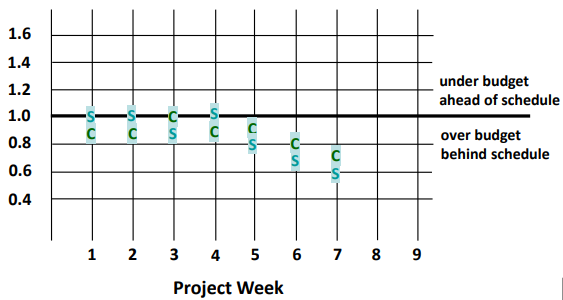
\includegraphics[width=\textwidth]{document/img/performance-indices-3.png}
		\caption{Indici di performance \#3}
		\label{perfind3}
	\end{subfigure}
	\hfill
	\begin{subfigure}[b]{0.45\textwidth}
		\centering
		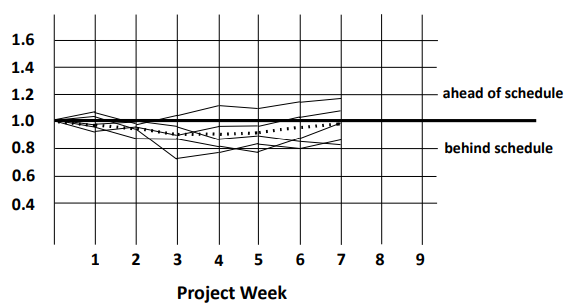
\includegraphics[width=\textwidth]{document/img/performance-indices-4.png}
		\caption{Indici di performance \#4}
		\label{perfind4}
	\end{subfigure}
\end{figure}

\subsection{Gestire la Scope Bank}
Si predispone un “deposito” iniziale di una certa percentuale del tempo complessivamente necessario (e.g., 5-10\%).
Il tempo necessario per processare e integrare una richiesta di modifica dello scope è attinto dalla Scope Bank.
Per aggiungere tempo alla Scope Bank è necessario rimuovere delle funzionalità/feature e depositare presso la Scope Bank il tempo che sarebbe stato richiesto per il loro sviluppo.
Se risparmiamo del tempo nell’esecuzione di qualche attività, si può aggiungere alla Scope Bank.
Il committente dovrebbe continuamente ridefinire le priorità del contenuto della Scope Bank.
\subsection{Costruire e mantenere l’Issues Log}
Durante l'esecuzione accadono molte disgrazie. L’Issues Log è un documento che contiene tutti i problemi che sono emersi durante il progetto e che ancora non sono stati risolti, per cui è molto dinamico.
La risoluzione dei problemi riportati nell’issues log è importante per la continuazione e il successo del progetto.
Le informazioni contenute nell’issues log possono essere le seguenti:
\begin{itemize}
	\item \textbf{ID Number}: In questo modo possiamo identificare in modo univoco il problema anche in altra documentazione;
	\item \textbf{Date logged}: Fornisce molte indicazioni e permette anche di ritrovarlo facilmente;
	\item \textbf{Descrizione del problema};
	\item \textbf{Descrizione dell’impatto sul progetto se non sarà risolto};
	\item \textbf{Definizione del “proprietario” del problema (problem owner)};
	\item \textbf{Azione che deve essere intrapresa per risolvere il problema};
	\item \textbf{Le descrizioni di tutti gli attempt fatti per poter risolvere il problema};
	\item \textbf{Stato}: Per esempio se è ancora da risolvere, in lavorazione, etc.;
	\item \textbf{Esito}.
\end{itemize}

\subsection{Gestire i Project Status Meetings}
Tutta la reportistica viene utilizzata e discussa in dei meeting appositi.
Per poter monitorare e controllare lo stato di avanzamento del progetto è necessario raccogliere le informazioni necessarie dal team.
Un valido strumento sono i Project Status Meeting che devono essere effettuati con cadenza periodica (e.g., giornaliera, settimanale, etc.). Valgono le stesse best practice di tutte le altre riunioni che sono già state discusse. Esistono diversi tipi di Project Status Meeting.

\subsubsection{15 Minutes Daily Status Meeting}
Partecipa l’intero team o solo i task manager responsabili dei task in lavorazione. Solitamente sono riunioni in cui tutti stanno in piedi. Un facilitatore potrebbe essere molto utile e può essere interpretato da uno dei partecipanti. Deve essere riportato sinteticamente lo stato di ciascun task:
\begin{itemize}
	\item “in schedula”;
	\item “in anticipo rispetto alla schedula” (specificando di quanto);
	\item “in ritardo rispetto alla schedula” (specificando di quanto e se c’è bisogno di aiuto).
\end{itemize}
Dopodiché si procede con l'aggiornamento della Scope Bank e con l'aggiornamento dell’Issues Log. Questo meeting viene utilizzato per capire come sta andando generalmente il progetto. La discussione più approfondita degli Issues deve essere affrontata in riunioni apposite.

\subsubsection{Problem Management Meeting}
Si tratta di riunioni che si tengono se si presenta un problema in cui è necessario l'intervento di più persone. Devono partecipare solo i membri del team che sono direttamente coinvolti. Va concordata la definizione del problema (non sempre infatti è esattamente chiaro quale sia il problema in primo luogo) e chi è il proprietario del problema. Si effettua del Brainstorming per cercare di trovare la soluzione del problema, si assegna una priorità alle soluzioni individuate e si aggiorna l’Issues Log (specificando se si è trovata una soluzione o aggiungendo dettagli). Solo se necessario si pianifica il prossimo meeting.

\subsection{Definire una Problem Escalation Strategy}
Per capire quale sia il problema a volte è necessaria una escalation, ovvero "fittare" la soluzione dentro al triangolo dello scope. L'implementazione di una soluzione infatti implica l'utilizzo di tempo, risorse, o costi aggiuntivi.
\centeredImage{document/img/problem-escalation-strategy.png}{Problem Escalation Strategy}{0.4}

\noindent Nella definizione della strategia di risoluzione dei problemi si possono individuare tre livelli, ovvero tre step dell'escalation:
\begin{itemize}
	\item \textbf{Project Manager-Based Strategies}: La figura che si interpella è il Project Manager. Potrebbe capire che non è richiesta nessuna azione in quanto il problema si risolverà da solo. In alternativa il project manager potrebbe esaminare le relazioni di dipendenza, riorganizzare la schedula e riassegnare le risorse.
	\item \textbf{Resource Manager-Based Strategies}: La figura da interpellare è il Resource Manager (potrebbe essere anche un senior manager). In questo caso è necessario negoziare per delle risorse aggiuntive.
	\item \textbf{Client-Based Strategies}: La figura da interpellare è il cliente. In questo caso si negozia un approccio basato su rilasci multipli, si richiede un’estensione della schedula o una modifica dello scope.
\end{itemize}

\subsubsection{Escalation Strategy Hierarchy}
L'escalation si compone quindi in una serie di step da affrontare in ordine:
\begin{itemize}
	\item Verificare se è possibile se sono richieste azioni (e.g., gli slack presenti nella schedula sono sufficienti a risolvere il problema);
	\item Esaminare le dipendenze di tipo Finish-to-Start (FS) per identificare delle opportunità di compressione della schedula;
	\item Riassegnare delle risorse dai task che non sono nel critical-path per contrastare il ritardo (slippage);
	\item Negoziare risorse aggiuntive;
	\item Negoziare una strategia che preveda dei rilasci multipli;
	\item Richiedere al cliente un’estensione della schedula;
	\item Richiedere al cliente una modifica di scope.
\end{itemize}

\subsection{Acquisire l’approvazione a chiudere il progetto}
Quando tutti i criteri previsti per l’accettazione della soluzione sono stati soddisfatti, il committente non può che essere contento e il progetto può entrare nella fase di chiusura.
